\documentclass[11pt,a4paper]{article}
\usepackage[margin=1in]{geometry}
\usepackage{amsmath,amssymb,amsthm,mathtools,bm}
\usepackage{enumitem}
\usepackage{booktabs}
\usepackage{array}
\usepackage{xcolor}
\usepackage{hyperref}
\usepackage{tikz}
\usetikzlibrary{arrows.meta,positioning,calc,decorations.pathreplacing,shapes.geometric}
\hypersetup{colorlinks=true,linkcolor=blue,urlcolor=blue,citecolor=blue}
\setlist[itemize]{leftmargin=2em,itemsep=0.3em,topsep=0.35em}
\setlist[enumerate]{leftmargin=2.2em,itemsep=0.3em,topsep=0.35em}

\newcommand{\R}{\mathbb{R}}
\newcommand{\N}{\mathbb{N}}
\newcommand{\ReLU}{\operatorname{ReLU}}
\newcommand{\Conv}{\operatorname{Conv}}
\newcommand{\Span}{\operatorname{span}}
\newcommand{\dd}{\,\mathrm{d}}
\newcommand{\Th}{\mathcal{T}_h}
\newcommand{\Vh}{V_h}
\newcommand{\Ah}{A_{\mathrm{Hat}}}
\newcommand{\Ar}{A_{\mathrm{ReLU}}}

\definecolor{titleblue}{RGB}{22,74,135}
\definecolor{softblue}{RGB}{235,244,255}
\definecolor{softgray}{RGB}{245,245,245}

\theoremstyle{definition}
\newtheorem{definition}{Definition}[section]
\newtheorem{example}{Example}[section]
\theoremstyle{plain}
\newtheorem{theorem}{Theorem}[section]
\theoremstyle{remark}
\newtheorem{remark}{Remark}[section]
\theoremstyle{plain}
\newtheorem{proposition}{Proposition}[section]
\newcommand{\boxnote}[1]{%
  \vspace{0.5em}
  \noindent\colorbox{softblue}{\parbox{0.965\linewidth}{#1}}
  \vspace{0.5em}
}

\title{\textbf{Lecture Notes: Deep Neural Networks and Finite Element Methods}}

\begin{document}
\maketitle
\tableofcontents
\newpage

\section*{Note on the Source}
\addcontentsline{toc}{section}{Note on the Source}
These notes are organized from the visible content in the classroom PPT photos. A few formulas were partially covered by the instructor, the projection interface, or the camera angle; in those places, the statements are completed in the most natural way from context. The main theme of the lecture is the following chain of ideas: a hiring-score example motivates deep neural networks; one-dimensional finite element basis functions are then related to ReLU basis functions; finally, the discussion is extended to finite element meshes, barycentric coordinates, and nodal basis functions.

\section{Course Policies and Objectives}

\subsection{Course policies}
The course policy slide gives two main requirements:
\begin{itemize}
  \item Bring your name card to every class.
  \item Assignments will be given after each class and are due before the next class. The submission format is a PDF file sent to \texttt{ai@multigrid.org}.
\end{itemize}

\subsection{Objectives of the course}
The course objectives can be summarized as follows:
\begin{enumerate}
  \item To provide a mathematical understanding of how and why deep learning works.
  \item To provide hands-on programming experience with popular and core deep learning models, including
  \begin{itemize}
    \item deep neural networks;
    \item convolutional neural networks;
    \item Transformers;
    \item and other related models.
  \end{itemize}
\end{enumerate}

\section{Activation functions}

\subsection{A linear score based on two factors}

Suppose a candidate is described by two factors:
\[
  x_1=\text{experience (years)},\qquad x_2=\text{education (degree)}.
\]
Let
\[
  x=\begin{pmatrix}x_1\\x_2\end{pmatrix},
  \qquad
  W=\begin{pmatrix}w_1&w_2\end{pmatrix}.
\]
A linear score is then
\[
  \text{score}=w_1x_1+w_2x_2+b=Wx+b.
\]
For a binary hiring decision, one may apply a step function $H$:
\[
  y=H(Wx+b),
\]
where
\[
  y=1 \quad \text{means Yes},
  \qquad
  y=0 \quad \text{means No}.
\]

\begin{center}
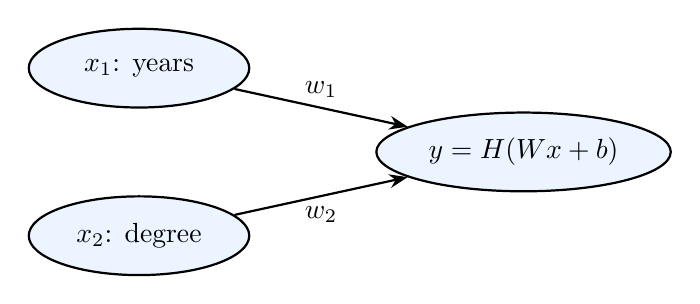
\begin{tikzpicture}[>=Stealth,node distance=2.0cm]
  \tikzstyle{oval}=[ellipse,draw,thick,minimum width=2.8cm,minimum height=1.0cm,fill=softblue]
  \node[oval] (x1) {$x_1$: years};
  \node[oval,below=1.1cm of x1] (x2) {$x_2$: degree};
  \node[oval,right=3.0cm of $(x1)!0.5!(x2)$] (y) {$y=H(Wx+b)$};
  \draw[->,thick] (x1) -- node[above] {$w_1$} (y);
  \draw[->,thick] (x2) -- node[below] {$w_2$} (y);
\end{tikzpicture}
\end{center}

\boxnote{The purpose of this example is to show that the basic building block of a neural network is still the linear function $Wx+b$. The difference is that a neural network repeatedly composes linear maps with nonlinear activation functions.}

\begin{definition}
[ReLU activation function]
\[
  \ReLU(x)=
  \begin{cases}
    x, & x>0,\\
    0, & x\le 0.
  \end{cases}
\]
\end{definition}

\textbf{Remark}. 
A refined decision model may be written as
\[
  y=W^1\ReLU(W^0x+b^0).
\]
For example, if $W^1=2000$, then
\[
  y=2000\,\ReLU(W^0x+b^0).
\]
The interpretation is
\[
  y>0 \quad \text{means Yes with salary},
  \qquad
  y\le 0 \quad \text{means No}.
\]

\subsection{A more refined multilayer model}
The model can be made more refined by introducing more input features, such as
\[
  x_1=\text{years},\quad
  x_2=\text{management},\quad
  x_3=\text{degree},\quad
  x_4=\text{university rank},\quad
  x_5=\text{GPA}.
\]
Let the original input be
\[
  x^0=x=\begin{pmatrix}x_1\\ \vdots \\ x_5\end{pmatrix}.
\]
The first layer may combine the raw variables into two intermediate concepts, such as experience and education:
\[
  x^1=\ReLU(W^0x+b^0),
\]
where the matrix displayed in the classroom has a grouped-feature structure, naturally written as
\[
  W^0=
  \begin{pmatrix}
    w_{11}^0 & w_{12}^0 & 0 & 0 & 0\\
    0 & 0 & w_{23}^0 & w_{24}^0 & w_{25}^0
  \end{pmatrix},
  \qquad
  b^0=\begin{pmatrix}b_1^0\\b_2^0\end{pmatrix}.
\]
Thus the first row extracts an ``experience'' feature mainly from years and management, while the second row extracts an ``education'' feature mainly from degree, university rank, and GPA. Subsequent layers continue this process:
\[
  x^2=\ReLU(W^1x^1+b^1),
  \qquad
  y=W^2x^2.
\]
This gives the transition from a simple linear model to a multilayer neural network.

\section{Deep Neural Networks: Linear Maps, Activations, and Composition}

The lecture summarizes the construction of a deep neural network function as follows:
\begin{enumerate}
  \item Start from a linear function:
  \[
    W^0x+b^0.
  \]
  \item Compose it with an activation function:
  \[
    x^1=\sigma(W^0x+b^0).
  \]
  \item Compose it with another linear function:
  \[
    W^1x^1+b^1.
  \]
  \item Compose again with the activation function:
  \[
    x^2=\sigma(W^1x^1+b^1).
  \]
  \item Attach another linear output layer:
  \[
    f(x;\theta)=W^2x^2+b^2.
  \]
\end{enumerate}

\begin{definition}[Neural Network]
    For a network with $\ell$ hidden layers, we may write
\[
  x^0=x,
  \qquad
  x^{k+1}=\sigma(W^kx^k+b^k),\quad k=0,1,\ldots,\ell-1,
\]
where $\sigma$ is an activation function and the final output is
\[
  f(x;\theta)=W^\ell x^\ell+b^\ell.
\]
Here
\[
  \theta=\{W^0,b^0,W^1,b^1,\ldots,W^\ell,b^\ell\}
\]
denotes all trainable parameters.
\end{definition}


Now we use a simple example to see what is learning for an NN. Suppose the training set consists of $N$ employees:
\[
  p^i,\quad i=1,2,\ldots,N.
\]
Each employee has an input feature vector
\[
  x^i=\begin{pmatrix}x_1^i\\x_2^i\end{pmatrix},
\]
where, for example, $x_1^i$ denotes experience and $x_2^i$ denotes education. The label is
\[
  y^i\in\{0,1,2,3,4\},
\]
with the interpretation
\[
  0:\text{bad},\quad
  1:\text{fair},\quad
  2:\text{good},\quad
  3:\text{very good},\quad
  4:\text{excellent}.
\]

The model displayed in class has the form
\[
  f(x,\theta)=w^2\sigma\bigl(w^1\sigma(w^0x+b^0)+b^1\bigr).
\]
The goal of learning is to find parameters $\theta=(w,b)$ such that
\[
  f(x^i,\theta)\approx y^i.
\]
Equivalently, one solves the empirical risk minimization problem
\[
  \min_\theta L(\theta)
  =\min_\theta \frac{1}{N}\sum_{i=1}^N
  \bigl|f(x^i,\theta)-y^i\bigr|^2.
\]
The optimal parameter is denoted by
\[
  \theta^*=\arg\min_\theta L(\theta).
\]
For a new candidate $x^{\mathrm{new}}$, the prediction is
\[
  f(x^{\mathrm{new}},\theta^*).
\]

\boxnote{Thus, in this example, ``learning from data'' means using training samples to determine the network parameters, minimizing the training error, and then applying the learned parameters to predict the output for a new sample.}



\subsection*{Exercises: Gradient Descent and Linear Regions}
\addcontentsline{toc}{subsection}{Exercises: Gradient Descent and Linear Regions}
\begin{enumerate}[label=\textbf{Exercise \arabic*.},leftmargin=2.6em]
  \item \textbf{Energy estimate for gradient descent.}
  Let $F:\mathbb R^d\to\mathbb R$ be continuously differentiable and strictly convex. Assume that $\nabla F$ is $L$-Lipschitz continuous, namely
  \[
    \|\nabla F(x)-\nabla F(y)\|\le L\|x-y\|,\qquad x,y\in\mathbb R^d,
  \]
  and assume that $F$ has a minimizer $u\in\mathbb R^d$. For arbitrary $u^0\in\mathbb R^d$, define
  \[
    u^m=u^{m-1}-\tau \nabla F(u^{m-1}),\qquad m=1,2,\ldots,
  \]
  where $0<\tau\le L^{-1}$. Prove that $u$ is the unique minimizer of $F$ and that, for every $m\ge1$,
  \[
    F(u^m)-F(u)\le \frac{\|u^0-u\|^2}{2\tau m}.
  \]

  \item \textbf{Linear regions of ReLU networks.}
  For $\sigma=\ReLU$, randomly sample parameters for $u\in\Sigma^\sigma_{n_1:L}$ and plot the linear regions of neural networks on $[-1,1]^2$ for the two cases $n_{1:L}=10$, $L=1$ and $L=2$.
\end{enumerate}

\section{Finite Element Discretization: From Function Spaces to Linear Systems}

Here we consider to use the finite element method to solve the Poisson equation
\[
-u''(x)  = f(x), \quad x\in(0,1)
\]
with $u(0) = 0, u'(1) = 0$.
\begin{definition}
    [Finite Element Space]
Suppose the finite element space satisfies
\[
  \Vh=\Span\{\varphi_1,\ldots,\varphi_{N+1}\}.
\]
A finite element approximation can be written as
\[
  u_h=\sum_{i=1}^{N+1}\alpha_i\varphi_i.
\]
If $f$ is the goal approximation, then for some bilinear form $a$ we have:
\[
  \sum_{j=1}^{N+1} a(\varphi_j,\varphi_i)\alpha_j=a(f,\varphi_i),
  \qquad i=1,\ldots,N+1.
\]
Equivalently,
\[
  A\alpha=b.
\]
Here
\[
  A=\{a(\varphi_j,\varphi_i)\}_{i,j=1}^{N+1}
  \in \R^{(N+1)\times(N+1)}
\]
is called the stiffness matrix, and 
\end{definition}

\subsection{Hat basis and ReLU basis}

\begin{definition}
    [Hat Basis] On a one-dimensional uniform grid, the standard linear finite element space uses hat basis functions. Each hat basis function takes value $1$ at one node, decreases linearly to $0$ at adjacent nodes, and is a piecewise linear function.
\end{definition}

The ReLU functions
\[
  r_i(x)=\ReLU(x-x_i)
\]
are piecewise linear. The central one-dimensional identity is
\[
  \phi(x)=1\cdot \ReLU(x)-2\cdot \ReLU(x-1)+1\cdot \ReLU(x-2).
\]
More generally, if the mesh size is $h$ and the nodes are $x_i$, then a local hat basis function can be written as a shifted and scaled combination of ReLU functions:
\[
  \varphi_i(x)
  =\ReLU\left(\frac{x-x_{i-1}}{h}\right)
  -2\ReLU\left(\frac{x-x_i}{h}\right)
  +\ReLU\left(\frac{x-x_{i+1}}{h}\right).
\]

\begin{proposition}
    One-dimensional finite element space can be regarded as a special shallow ReLU network space.
\end{proposition}
\begin{proof}
    On a fixed uniform grid, one may write
\[
  \Vh
  =\left\{\sum_{i=1}^{N+1} a_i\varphi_i(x)\right\}
  =\left\{\sum_{i=1}^{N+1} a_i\ReLU(w_i x+b_i)\right\},
\]
where one typical choice of parameters is
\[
  w_i=\frac{1}{h},
  \qquad
  b_i=-\frac{x_{i-1}}{h}.
\]
If the ReLU parameters $w_i,b_i$ are also allowed to vary freely, we obtain the one-dimensional shallow ReLU network space
\[
  \Sigma_n^{\ReLU}
  =\left\{
  \sum_{i=1}^n a_i\ReLU(w_ix+b_i):
  w_i,b_i\in\R,
  i=1,\ldots,n
  \right\}.
\]
The breakpoint of each ReLU unit is
\[
  x_i=-\frac{b_i}{w_i}.
\]
Therefore, a shallow ReLU network can be interpreted as a finite element function on a movable grid.


\end{proof}

\begin{theorem}
In the one-dimensional setting, with a suitable ordering and compatible boundary conditions, the stiffness matrix associated with the hat basis and the matrix associated with the ReLU basis satisfy
\[
  \Ar=\Ah^{-1}.
\]
Consequently, if $(\lambda_{k,\Ah},\xi_{\Ah}^k)$ is an eigenpair of $\Ah$, that is,
\[
  \Ah\xi_{\Ah}^k=\lambda_{k,\Ah}\xi_{\Ah}^k,
\]
then, after identifying the two coordinate representations in the same vector space,
\[
  \Ar\xi_{\Ah}^k=\lambda_{k,\Ah}^{-1}\xi_{\Ah}^k.
\]
\end{theorem}

\begin{proof}
    In the one-dimensional setting, we know
    \[\phi_i = r_{i-1} - 2r_i + r_{i+1}\]
    and hence
    \[
        \phi_i ' = \dfrac{1}{h}(\chi_{(x_{i-1},\infty)} - 2\chi_{(x_i,\infty)}+\chi_{(x_{i+1},\infty)})
    \]
    We have
    \[
    A_{Hat}=\frac1{h^2} K,
    \]
    where
    \[
    K=
    \begin{pmatrix}
    2 & -1 \\
    -1 & 2 & -1 \\
    & \ddots & \ddots & \ddots \\
    && -1 & 2 & -1 \\
    &&& -1 & 1 \end{pmatrix}
\]
and then let $h^2 r_i$ to be the new basis $\gamma_i$ and we have 
\[
\int \gamma_i'\gamma_j' = h(i\vee j)
\]

Then we may compute
\[
A_{\text{Hat}}A_{\text{ReLU}} = I
\]
\end{proof}

\begin{definition}[Finite element partition]
Let $\Omega\subset \R^d$ be a bounded domain. A finite element partition, also called a mesh or grid and denoted by $\Th$, is a collection of $d$-simplices satisfying:
\begin{enumerate}
  \item Covering by closures:
  \[
    \overline{\Omega}=\bigcup_{\tau\in\Th}\tau.
  \]
  \item Disjoint interiors: if $\tau_1,\tau_2\in\Th$ and $\tau_1\ne \tau_2$, then
  \[
    \tau_1^\circ\cap \tau_2^\circ=\varnothing.
  \]
\end{enumerate}
\end{definition}

A $d$-simplex is the simplest element in $d$ dimensions: an interval in one dimension, a triangle in two dimensions, and a tetrahedron in three dimensions.

\section{Barycentric Coordinates}

Let $\tau\in\Th$ be an element with vertices
\[
  a_0,a_1,\ldots,a_d.
\]
Then
\[
  \tau=\Conv(a_0,\ldots,a_d).
\]
For any $x\in\tau$, there exist unique numbers
\[
  \lambda_0(x),\lambda_1(x),\ldots,\lambda_d(x)
\]
such that
\[
  x=\sum_{i=0}^d \lambda_i(x)a_i,
  \qquad
  \sum_{i=0}^d \lambda_i(x)=1,
  \qquad
  \lambda_i(x)\in[0,1].
\]
These numbers are called the barycentric coordinates of $x$ with respect to the element $\tau$.

The lecture also gives a geometric interpretation. Let $\tau_i(x)$ be the simplex obtained from $\tau$ by replacing the vertex $a_i$ with $x$. Then
\[
  \lambda_i(x)=\frac{|\tau_i(x)|}{|\tau|},
  \qquad i=0,\ldots,d.
\]
Here $|\tau|$ denotes the $d$-dimensional volume of the element; in two dimensions it is area, and in three dimensions it is volume.

\boxnote{Barycentric coordinates express any point $x$ inside an element as a linear interpolation of the vertices $a_0,\ldots,a_d$. On each element, the linear finite element basis functions are precisely these barycentric coordinate functions.}

\begin{definition}[Linear Nodal Functions for Partition]
Let
\(
  \{x_i\}_{i=1}^{n_h}
\)
be the set of nodes of the partition $\Th$. The linear finite element space $\Vh$ has a natural set of basis functions
\(
  \{\varphi_i\}_{i=1}^{n_h}\subset \Vh,
\)
called nodal basis functions, satisfying the interpolation property
\[
  \varphi_i(x_j)=\delta_{ij}.
\]
In one dimension, $\varphi_i$ is the hat function peaked at the node $x_i$. On a two-dimensional triangular mesh, $\varphi_i$ is a piecewise linear tent function with peak value $1$ at the node $x_i$. It is nonzero on elements adjacent to $x_i$ and zero on elements not touching $x_i$.
\end{definition}

\section{Weak Formulation, Galerkin Approximation, and FEM Error Estimates}

\subsection{Weak formulation of the model problem}
Consider again
\[
  -u''=f \quad \text{in }(0,1),
  \qquad
  u(0)=0,
  \qquad
  u'(1)=0.
\]
Let
\[
  V=\{v:[0,1]\to\R:\ v \text{ is continuous and piecewise smooth, and }v(0)=0\}.
\]
Multiplying the equation by a test function $v\in V$ and integrating by parts gives
\[
  \int_0^1-u''v\,\dd x
  =\int_0^1u'v'\,\dd x-\bigl[u'v\bigr]_0^1
  =\int_0^1u'v'\,\dd x.
\]
The boundary term vanishes because $v(0)=0$ and $u'(1)=0$. Thus the weak problem is
\[
  a(u,v)=\ell(v),\qquad \forall v\in V,
\]
where
\[
  a(u,v):=\int_0^1u'(x)v'(x)\,\dd x,
  \qquad
  \ell(v):=\int_0^1f(x)v(x)\,\dd x.
\]

\subsection{Galerkin method and energy minimization}
On the uniform grid
\[
  0=x_0<x_1<\cdots<x_{N+1}=1,
  \qquad
  x_j=\frac{j}{N+1},
  \qquad
  h=\frac{1}{N+1},
\]
define
\[
  V_h=\{v_h\in C([0,1]):v_h|_{[x_{j-1},x_j]}\in P_1,
  \ v_h(0)=0\}.
\]
The Galerkin approximation is the function $u_h\in V_h$ satisfying
\[
  a(u_h,v_h)=\ell(v_h),\qquad \forall v_h\in V_h.
\]
Introduce the energy functional
\[
  J(v)=\frac12a(v,v)-\ell(v).
\]
Then the continuous and discrete solutions are characterized by
\[
  u=\arg\min_{v\in V}J(v),
  \qquad
  u_h=\arg\min_{v_h\in V_h}J(v_h).
\]
Indeed, the first variation of $J$ at $u$ in the direction $v$ is
\[
  \frac{\dd}{\dd t}J(u+tv)\bigg|_{t=0}=a(u,v)-\ell(v).
\]

\begin{theorem}[C\'ea's lemma in the energy norm]
Assume that $a(\cdot,\cdot)$ is symmetric and defines an inner product on $V$. If $u$ and $u_h$ solve the continuous and Galerkin problems, then
\[
  \|u-u_h\|_a
  =\inf_{v_h\in V_h}\|u-v_h\|_a,
  \qquad
  \|v\|_a^2:=a(v,v).
\]
\end{theorem}

\begin{proof}
Galerkin orthogonality gives
\[
  a(u-u_h,v_h)=0,\qquad \forall v_h\in V_h.
\]
For arbitrary $v_h\in V_h$,
\[
  \|u-u_h\|_a^2
  =a(u-u_h,u-v_h)+a(u-u_h,v_h-u_h)
  =a(u-u_h,u-v_h).
\]
By Cauchy--Schwarz,
\[
  \|u-u_h\|_a\le \|u-v_h\|_a.
\]
Taking the infimum over $v_h\in V_h$ proves the result.
\end{proof}

Combining this best-approximation property with the interpolation estimate for continuous piecewise linear functions gives
\[
  \|u-u_h\|_{H^1(0,1)}\lesssim h\,|u|_{H^2(0,1)}.
\]

\subsection*{Exercises: One-Dimensional FEM, ReLU Basis, and Gradient Descent}
  \textbf{Poisson equation with hat and ReLU bases.}
  Solve the Poisson equation on $[0,1]$:
  \[
    -u''=f\quad\text{in }(0,1),
    \qquad u(0)=0,
    \qquad u'(1)=0.
  \]
  Let
  \[
    f(x)=\frac94\pi^2\sin\left(\frac32\pi x\right),
    \qquad
    u(x)=\sin\left(\frac32\pi x\right).
  \]
  Apply FEM with the hat basis and the ReLU basis separately. Then solve the corresponding linear systems by the gradient descent method and plot the residual functions at iterations
  \[
    1,\\ 50,\\ 500,\\ 5000.
  \]

\section{High-Dimensional Linear FEM and ReLU Networks}

\subsection{Piecewise linearity and local geometry}
A ReLU network is continuous and piecewise affine on a polyhedral partition of its input domain. Consequently,
\[
  \Sigma^1_{n_1:L}\subset \{\text{continuous piecewise linear functions}\}\subset H^1(\Omega).
\]
Conversely, linear finite element basis functions can be represented by ReLU networks. The basic algebraic identities are
\[
  x=\ReLU(x)-\ReLU(-x),
  \qquad
  |x|=\ReLU(x)+\ReLU(-x),
\]
and
\[
  \min(a,b)=\frac{a+b-|a-b|}{2}.
\]
Equivalently,
\[
  \min(a,b)=v\cdot\ReLU\!\left(W\begin{pmatrix}a\\b\end{pmatrix}\right),
\]
where
\[
  v=\frac12(1,-1,-1,-1),
  \qquad
  W=
  \begin{pmatrix}
  1&1\\
  -1&-1\\
  1&-1\\
  -1&1
  \end{pmatrix}.
\]

Let $v$ be a vertex of a simplicial mesh and let $P_v$ be its vertex patch. For every element $\tau_i\subset P_v$, let $g_i$ be the global affine function agreeing with the nodal basis function $\varphi_v$ on $\tau_i$. If the patch $P_v$ is convex, then
\[
  \varphi_v(x)=\max\left\{0,\min_{i\in\mathcal N(v)}g_i(x)\right\}
  =\ReLU\left(\min_{i\in\mathcal N(v)}g_i(x)\right).
\]
The minimum of many affine functions can be evaluated by a binary tree of pairwise minimum operations. If $d_h$ is the maximal number of elements meeting at one vertex, this gives a depth of order
\[
  2+\lceil\log_2d_h\rceil.
\]
For a nonconvex patch, one decomposes or slightly enlarges it into convex pieces, constructs one local ReLU representation on each piece, and takes their maximum.

\begin{theorem}[Linear FEM represented by ReLU-DNN]
Let $V_h$ be a linear finite element space on a simplicial mesh and let $N$ be its number of degrees of freedom. Every $v_h\in V_h$ can be represented exactly by a ReLU deep neural network. One construction has depth
\[
  L=2+\lceil\log_2d_h\rceil
\]
and $O(d_hN)$ neurons, where $d_h$ is the largest number of elements sharing a vertex.
\end{theorem}

The updated slides also emphasize that a deeper and narrower construction can reduce the depth dependence to a quantity controlled by the simplex dimension, using a balanced max--min representation of each local basis function.



\subsection*{Exercises: ReLU Identities and Max-Min Constructions}
\addcontentsline{toc}{subsection}{Exercises: ReLU Identities and Max-Min Constructions}
\begin{enumerate}[label=\textbf{Exercise \arabic*.},leftmargin=2.6em]
  \item \textbf{Pairwise minimum and product identities.}
  For any $(x,y)\in\mathbb R^2$, prove that
  \[
    \min\{x,y\}=a_1\ReLU\left(W\begin{pmatrix}x\\y\end{pmatrix}\right)
  \]
  and
  \[
    xy=a_2\ReLU^2\left(W\begin{pmatrix}x\\y\end{pmatrix}\right),
  \]
  where $\ReLU$ and $\ReLU^2$ act componentwise, and
  \[
    W=
    \begin{pmatrix}
      1&1\\
      -1&-1\\
      1&-1\\
      -1&1
    \end{pmatrix},
    \qquad
    a_1=\frac12(1,-1,-1,-1),
    \qquad
    a_2=\frac14(1,1,-1,-1).
  \]
\end{enumerate}

\section{Universal Approximation by Shallow Networks}

\begin{theorem}[Weierstrass approximation theorem]
Let $\Omega\subset\R^d$ be compact. For every $f\in C(\Omega)$ there exists a sequence of polynomials $p_n$ such that
\[
  \lim_{n\to\infty}\max_{x\in\Omega}|f(x)-p_n(x)|=0.
\]
\end{theorem}

For an activation function $\sigma$, define the shallow network class
\[
  \Sigma_n^\sigma
  =\left\{\sum_{i=1}^na_i\sigma(w_i\cdot x+b_i):
  w_i\in\R^d,\ b_i,a_i\in\R\right\},
\]
and let $\Sigma^\sigma=\bigcup_{n\ge1}\Sigma_n^\sigma$.

\begin{theorem}[Universal approximation criterion]
In the standard shallow-network setting on a compact domain, the uniform closure of $\Sigma^\sigma$ contains $C(\Omega)$ if and only if $\sigma$ is not a polynomial.
\end{theorem}

For a smooth non-polynomial activation, the main idea is particularly transparent. Since finite differences of ridge functions remain in the closure of the network class,
\[
  \frac{\sigma((w+he_j)\cdot x+b)-\sigma(w\cdot x+b)}{h}
  \longrightarrow x_j\sigma'(w\cdot x+b).
\]
At $w=0$, if $\sigma'(b)\neq0$, this produces $x_j$. More generally,
\[
  D_w^\alpha\sigma(w\cdot x+b)=x^\alpha\sigma^{(|\alpha|)}(w\cdot x+b).
\]
Because a non-polynomial smooth function has nonzero derivatives of arbitrarily high order at suitable points, all monomials, and hence all polynomials, belong to the closure. The Weierstrass theorem then gives density in $C(\Omega)$. For nonsmooth activations, the same conclusion is obtained by a distributional or finite-difference argument.

If $\sigma$ is a polynomial of degree $m$, the conclusion fails for a fixed depth: compositions and linear combinations produce polynomials of bounded degree depending only on $m$ and the depth, so the resulting class cannot be dense in $C(\Omega)$.



\subsection*{Exercises: Universal Approximation}
\addcontentsline{toc}{subsection}{Exercises: Universal Approximation}
\begin{enumerate}[label=\textbf{Exercise \arabic*.},leftmargin=2.6em]
  \item \textbf{Non-polynomial activation and density.}
  Let $\Omega\subset\mathbb R^d$, and let $\sigma:\mathbb R\to\mathbb R$ be a Riemann integrable non-polynomial function. Define
  \[
    \Sigma^\sigma
    =\left\{
      \sum_{i=1}^n a_i\sigma(w_i\cdot x+b_i):
      a_i,b_i\in\mathbb R,
      \ w_i\in\mathbb R^d,
      \ n\ge0
    \right\}.
  \]
  Prove that $\Sigma^\sigma$ is dense in $C(\Omega)$ in the uniform norm.

  \item \textbf{Weierstrass theorem and polynomial activations.}
  Let $\Omega\subset\mathbb R^d$ be closed and bounded.
  \begin{enumerate}[label=(\alph*)]
    \item State the Weierstrass approximation theorem.
    \item Suppose $\sigma$ is a polynomial. Determine whether $\Sigma^\sigma_{n_{1:L}}$ is dense in $C(\Omega)$.
  \end{enumerate}
\end{enumerate}

\section{High-Order Lagrange Finite Elements}

\subsection{Local nodes and barycentric indices}
For a simplex $\tau$ with barycentric coordinates $\lambda_0,\ldots,\lambda_d$, define the degree-$k$ interpolation nodes
\[
  X_k(\tau)
  =\left\{p\in\tau:\lambda_i(p)\in
  \left\{0,\frac1k,\ldots,\frac{k-1}{k},1\right\},\ i=0,\ldots,d\right\}.
\]
For $p=x_\alpha\in X_k(\tau)$, its barycentric index is
\[
  \alpha=(\alpha_0,\ldots,\alpha_d),
  \qquad
  \alpha_i=k\lambda_i(p)\in\N,
  \qquad
  \sum_{i=0}^d\alpha_i=k.
\]
The number of nodes is
\[
  |X_k(\tau)|=\binom{d+k}{k}=\dim P_k(\tau).
\]

\begin{theorem}[Local Lagrange basis formula]
For $p=x_\alpha\in X_k(\tau)$, the associated nodal basis function is
\[
  \varphi_p(x)
  =\frac1{\alpha!}
  \prod_{i=0}^d\prod_{j=0}^{\alpha_i-1}
  \bigl(k\lambda_i(x)-j\bigr),
  \qquad
  \alpha!:=\prod_{i=0}^d\alpha_i!.
\]
It satisfies
\[
  \varphi_p(q)=\delta(p,q),\qquad q\in X_k(\tau).
\]
\end{theorem}

\begin{proof}
The total degree is $\sum_i\alpha_i=k$, so $\varphi_p\in P_k(\tau)$. Let $q=x_\beta\neq p$. Since $\sum_i\alpha_i=\sum_i\beta_i=k$, there is an index $i$ with $\beta_i<\alpha_i$. The factor with $j=\beta_i$ then vanishes at $q$, and hence $\varphi_p(q)=0$. At $p$,
\[
  k\lambda_i(p)=\alpha_i,
\]
so the product equals $\prod_i\alpha_i!=\alpha!$. The normalization gives $\varphi_p(p)=1$.
\end{proof}

\subsection{Sub-simplices and global basis functions}
Let $\Delta_\ell(\tau)$ denote the set of $\ell$-dimensional sub-simplices of $\tau$. For a mesh,
\[
  \Delta_\ell(\Th)=\bigcup_{\tau\in\Th}\Delta_\ell(\tau).
\]
The global interpolation nodes decompose according to the smallest-dimensional sub-simplex containing them:
\[
  X_k(\Th)=\bigsqcup_{\ell=0}^dX_k^\ell(\Th),
  \qquad
  X_k^\ell(\Th)=\bigsqcup_{f\in\Delta_\ell(\Th)}X_k(\mathring f).
\]

Suppose $p$ lies in the interior of an $\ell$-dimensional sub-simplex $f$ with vertices
\[
  v_0^f,\ldots,v_\ell^f.
\]
Let $\varphi_{v_i^f}$ denote the global piecewise linear hat function associated with $v_i^f$. Then the high-order global basis function can be written without an element-by-element definition as
\[
  \varphi_p(x)
  =\frac1{\alpha!}
  \prod_{i=0}^\ell\prod_{j=0}^{\alpha_i-1}
  \bigl(k\varphi_{v_i^f}(x)-j\bigr).
\]
Outside all elements containing $f$, at least one factor $\varphi_{v_i^f}$ vanishes. On an element containing $f$, the linear hat functions coincide with the corresponding barycentric coordinates, so the formula reduces to the local Lagrange formula.



\subsection*{Exercises: High-Order Lagrange Basis Functions}
\addcontentsline{toc}{subsection}{Exercises: High-Order Lagrange Basis Functions}
\begin{enumerate}[label=\textbf{Exercise \arabic*.},leftmargin=2.6em]
  \item \textbf{Verification of the barycentric nodal basis formula.}
  Denote
  \[
    X_k(\tau)=\left\{p\in\tau:
    \lambda_i(p)\in\left\{0,\frac1k,\ldots,\frac{k-1}{k},1\right\},
    \ i=0,1,\ldots,d\right\}.
  \]
  For a node $p=x_\alpha\in X_k(\tau)$, define its barycentric index by
  \[
    \alpha=(\alpha_0,\alpha_1,\ldots,\alpha_d),
    \qquad
    \alpha_i=k\lambda_i(p)\in\mathbb N,
    \qquad
    \sum_{i=0}^d\alpha_i=k.
  \]
  Verify that the functions
  \[
    \varphi_p(x)
    =\frac1{\alpha!}
    \prod_{i=0}^d\prod_{j=0}^{\alpha_i-1}
    \bigl(k\lambda_i(x)-j\bigr),
    \qquad p=x_\alpha\in X_k(\tau),
  \]
  satisfy the nodal property
  \[
    \varphi_p(q)=\delta(p,q)=
    \begin{cases}
      1, & q=p,\\
      0, & q\ne p,
    \end{cases}
    \qquad q\in X_k(\tau).
  \]
\end{enumerate}

\section{ReLU$^k$ Networks and High-Order FEM}

Define
\[
  \sigma_k(t)=\ReLU(t)^k.
\]
A ReLU$^k$ network is piecewise polynomial. Its local polynomial degree grows under composition, and a depth-$L$ construction can represent polynomials of degree up to $k^L$.

\begin{proposition}[Ridge representation of polynomials]
Every polynomial $p\in P_k(\R^d)$ can be written as a finite linear combination of ridge polynomials
\[
  (w\cdot x+b)^k.
\]
\end{proposition}

The basic identity
\[
  t^k=\sigma_k(t)+(-1)^k\sigma_k(-t)
\]
then represents degree-$k$ ridge polynomials by ReLU$^k$ neurons. Repeated composition represents higher polynomial degrees.

For $k=2$, multiplication is available exactly. For every $(x,y)\in\R^2$,
\[
  xy=\frac14(1,1,-1,-1)
  \ReLU^2\!\left(
  \begin{pmatrix}
  1&1\\
  -1&-1\\
  1&-1\\
  -1&1
  \end{pmatrix}
  \begin{pmatrix}x\\y\end{pmatrix}
  \right).
\]
Thus a network using both ReLU and ReLU$^2$ can combine piecewise linear functions with exact multiplications.

\begin{theorem}[Representation of Lagrange finite elements]
Every $P_k$ Lagrange finite element function on an arbitrary simplicial mesh can be represented exactly by a deep network whose activation at each neuron is a linear combination of ReLU and ReLU$^2$. With fixed width, the number of parameters can be chosen of order $O(N)$, where $N$ is the number of finite element degrees of freedom.
\end{theorem}

The mechanism is the global product formula for high-order basis functions: each high-order basis is a product of linear hat functions, linear hat functions are represented by ReLU-DNNs, and products are represented by ReLU$^2$ subnetworks.

\section{Quantitative Approximation by Shallow Neural Networks}

\subsection{Cosine networks and Fourier integral representation}
Let
\[
  \widehat u(w)=\int_{\R^d}u(x)e^{-2\pi i w\cdot x}\,\dd x
\]
and assume $\widehat u\in L^1(\R^d)$. Write
\[
  \widehat u(w)=|\widehat u(w)|e^{ib(w)},
  \qquad
  \lambda(w)=\frac{|\widehat u(w)|}{\|\widehat u\|_{L^1}}.
\]
Fourier inversion gives
\[
  u(x)
  =\int_{\R^d}\cos(2\pi w\cdot x+b(w))|\widehat u(w)|\,\dd w
  =\|\widehat u\|_{L^1}\,\mathbb E_\lambda[g(w,x)],
\]
where
\[
  g(w,x)=\cos(2\pi w\cdot x+b(w)).
\]
Let $w_1,\ldots,w_n$ be independent samples from $\lambda$. In the Hilbert space $L^2([0,1]^d)$,
\[
  \mathbb E\left\|
  \mathbb E g-\frac1n\sum_{i=1}^ng(w_i,\cdot)
  \right\|_{L^2}^2
  =\frac1n\left(
  \mathbb E\|g\|_{L^2}^2-\|\mathbb E g\|_{L^2}^2
  \right)
  \le\frac1n.
\]
Therefore at least one deterministic sample satisfies the same upper bound, and there exists a cosine network $u_n$ such that
\[
  \|u-u_n\|_{L^2([0,1]^d)}
  \le n^{-1/2}\|\widehat u\|_{L^1(\R^d)}.
\]
The condition $\widehat u\in L^1$ also implies that $u$ is bounded, continuous, and vanishes at infinity.

\subsection{Spectral Barron spaces}
For a bounded domain $\Omega$, define the spectral Barron norm
\[
  \|f\|_{\mathcal B_s(\Omega)}
  :=\inf_{\widetilde f|_\Omega=f}
  \int_{\R^d}(1+|\omega|)^s
  |\widehat{\widetilde f}(\omega)|\,\dd\omega.
\]
The infimum is over extensions to $\R^d$. If $f\in H^r(\R^d)$ with $r>d/2$, then the Fourier transform is integrable by Cauchy--Schwarz, so Sobolev regularity above the critical index implies a finite spectral Barron norm of order zero.

For sigmoidal activations on bounded domains, the classical Barron estimate has the form
\[
  \inf_{u_N\in\Sigma_N^\sigma}
  \|u-u_N\|_{L^2(\Omega)}
  \lesssim N^{-1/2}\|u\|_{\mathcal B_1(\Omega)}.
\]
The updated slides also record extensions to compactly supported and smooth activations, as well as Sobolev-norm estimates. For suitable $\sigma\in W^{m,\infty}_{\mathrm{loc}}$ with polynomial decay,
\[
  \inf_{u_N\in\Sigma_N^\sigma}
  \|u-u_N\|_{H^m(\Omega)}
  \lesssim N^{-1/2}\|u\|_{\mathcal B_{m+1}(\Omega)}.
\]
Under much weaker Fourier nondegeneracy assumptions on a bounded activation, one still obtains a slower bound of order $N^{-1/4}$.

For ReLU$^k$, the slides state two complementary estimates: a dimension-independent Monte Carlo rate under weaker spectral smoothness,
\[
  \inf_{u_N\in\Sigma_N^{\sigma_k}}
  \|u-u_N\|_{L^2(\Omega)}
  \lesssim N^{-1/2}\|u\|_{\mathcal B_{1/2}(\Omega)},
\]
and, for sufficiently large $s$,
\[
  \inf_{u_N\in\Sigma_N^{\sigma_k}}
  \|u-u_N\|_{L^2(\Omega)}
  \lesssim N^{-(k+1)}\log N\,\|u\|_{\mathcal B_s(\Omega)}.
\]
The first estimate requires less smoothness; the second uses greater smoothness to obtain a faster rate.



\subsection*{Exercises: Sampling Argument in $L^2$}
\addcontentsline{toc}{subsection}{Exercises: Sampling Argument in $L^2$}
\begin{enumerate}[label=\textbf{Exercise \arabic*.},leftmargin=2.6em]
  \item \textbf{Expected squared error of empirical averages.}
  Let $\Omega=[0,1]$. Consider a function $g:\Omega\times\mathbb R\to\mathbb R$ such that for every deterministic parameter $\theta\in\mathbb R$, the map $x\mapsto g(x,\theta)$ belongs to $L^2(\Omega)$. Suppose that $w$ is a real-valued random variable with probability density function $\lambda$. Draw i.i.d. samples $w_1,\ldots,w_n$ from this distribution and denote
  \[
    g_i(x)=g(x,w_i).
  \]
  \begin{enumerate}[label=(\alph*)]
    \item By the definition of expectation, derive the formula for
    \[
      \mu(x)=\mathbb E_w[g(x,w)]
    \]
    and for the expected $L^2$-norm squared error
    \[
      \mathbb E_n\left[
      \left\|\mu-\frac1n\sum_{i=1}^n g_i\right\|_{L^2(\Omega)}^2
      \right].
    \]
    \item Calculate the expectation and prove that
    \[
      \mathbb E_n\left[
      \left\|\mu-\frac1n\sum_{i=1}^n g_i\right\|_{L^2(\Omega)}^2
      \right]
      =\frac1n\left(
      \mathbb E_w\bigl[\|g(\cdot,w)\|_{L^2(\Omega)}^2\bigr]
      -\|\mu\|_{L^2(\Omega)}^2
      \right)
      \le \frac1n,
    \]
    under the normalization $\mathbb E_w\|g(\cdot,w)\|_{L^2(\Omega)}^2\le1$.
  \end{enumerate}
\end{enumerate}

\section{Variation Spaces and Barron Spaces}

\subsection{Dictionary and variation norm}
Let $G_\sigma\subset\R^{d+1}$ be compact and define the symmetric dictionary
\[
  D_\sigma
  =\{\pm\sigma(w\cdot x+b):(w,b)\in G_\sigma\}
  \subset L^2(\Omega).
\]
For a general bounded dictionary $D$ in a Hilbert space $H$, define
\[
  \Sigma_n(D)=\left\{\sum_{i=1}^na_ih_i:h_i\in D\right\}.
\]
The variation space is the linear space generated by the closed absolutely convex hull of $D$. Its norm can be written as the gauge
\[
  \|f\|_{V(D)}
  =\inf\left\{M>0:f\in M\,\overline{\operatorname{conv}}(D)\right\}.
\]
Equivalently, it is the infimum of the total coefficient mass over finite or limiting dictionary representations of $f$.

For ReLU$^k$, positive homogeneity permits normalization of the parameters. With $\widetilde x=(x,1)$ and
\[
  \theta=\frac{(w,b)}{\sqrt{|w|^2+b^2}}\in S^d,
\]
we have
\[
  \ReLU^k(w\cdot x+b)
  =\bigl(|w|^2+b^2\bigr)^{k/2}
  \ReLU^k(\theta\cdot\widetilde x).
\]
Thus the normalized parameter set can be taken to be the sphere $S^d$.

\begin{theorem}[Barron--Jones--Maurey]
Let $D$ be a bounded dictionary in a Hilbert space $H$, and set
\[
  |D|:=\sup_{h\in D}\|h\|_H.
\]
Then
\[
  \inf_{f_n\in\Sigma_n(D)}\|f-f_n\|_H
  \le |D|\,\|f\|_{V(D)}\,n^{-1/2}.
\]
Moreover, $f_n$ may be chosen with total coefficient mass at most $\|f\|_{V(D)}$.
\end{theorem}

\begin{proof}
It is enough to consider $\|f\|_{V(D)}\le1$. Given $\varepsilon>0$, choose
\[
  g=\sum_{i=1}^Na_ih_i,
  \qquad
  a_i\ge0,
  \qquad
  \sum_{i=1}^Na_i=1,
  \qquad
  \|f-g\|_H\le\varepsilon.
\]
Let a random variable $h$ take the value $h_i$ with probability $a_i$, and let $h_1^*,\ldots,h_n^*$ be independent copies. Then $\mathbb Eh=g$ and
\[
  \mathbb E\left\|g-\frac1n\sum_{j=1}^nh_j^*\right\|_H^2
  =\frac1n\left(\mathbb E\|h\|_H^2-\|\mathbb Eh\|_H^2\right)
  \le\frac{|D|^2}{n}.
\]
Hence one realization satisfies
\[
  \left\|g-\frac1n\sum_{j=1}^nh_j^*\right\|_H
  \le |D|n^{-1/2}.
\]
Combining this with $\|f-g\|_H\le\varepsilon$ and then letting $\varepsilon\downarrow0$ proves the unit-ball estimate. Scaling gives the general case.
\end{proof}

The exponent $1/2$ is optimal in the worst case over all dictionaries. For example, with $D=\{e_j\}_{j\ge1}\subset\ell^2$ and
\[
  f=\frac1{2n}\sum_{j=1}^{2n}e_j,
\]
any $n$-term approximation misses at least $n$ coordinates, giving an error bounded below by a constant multiple of $n^{-1/2}$.

\subsection{Barron space associated with an activation}
For $M>0$, define
\[
  \Sigma_{n,M}^\sigma
  =\left\{\sum_{i=1}^na_ih_i:
  h_i\in D_\sigma,
  \ \sum_{i=1}^n|a_i|\le M\right\}.
\]
The activation Barron space $B^\sigma(\Omega)$ is the closure, in $L^2(\Omega)$, of functions admitting uniformly bounded coefficient mass. Its norm is the smallest such mass. In this notation, the lecture theorem states that, for $\sigma\in L^\infty_{\mathrm{loc}}(\R)$,
\[
  u\in B^\sigma(\Omega)
  \quad\Longleftrightarrow\quad
  \text{there exists }M>0\text{ such that }
  \lim_{n\to\infty}
  \inf_{u_n\in\Sigma_{n,M}^\sigma}
  \|u-u_n\|_{L^2(\Omega)}=0.
\]
Furthermore,
\[
  \inf_{u_n\in\Sigma_{n,M}^\sigma}
  \|u-u_n\|_{L^2(\Omega)}
  \le Cn^{-1/2}\|u\|_{B^\sigma(\Omega)}.
\]

For the cosine dictionary, the Fourier integral representation shows that
\[
  \|u\|_{B^{\cos}}\le \|\widehat u\|_{L^1}.
\]
Thus the Fourier $L^1$ space is a concrete Barron space. For the $\tanh$ dictionary, one uses signed measures on a compact parameter domain:
\[
  u(x)=\int a(\theta)\tanh(w\cdot x+b)\,\dd\rho(\theta),
\]
with norm given by the infimum of the total variation of the representing signed measure. Unlike ReLU, $\tanh$ is not positively homogeneous, so the parameter normalization must be imposed through a compact parameter set rather than absorbed into the outer coefficient.



\subsection*{Exercises: Barron and Variation Spaces}
\addcontentsline{toc}{subsection}{Exercises: Barron and Variation Spaces}
\begin{enumerate}[label=\textbf{Exercise \arabic*.},leftmargin=2.6em]
  \item \textbf{$n^{-1/2}$ approximation rate in Barron spaces.}
  Let
  \[
    \Sigma_{n,M}^\sigma
    :=\left\{
      \sum_{i=1}^n a_i h_i:
      h_i\in D_\sigma,
      \ \sum_{i=1}^n |a_i|\le M
    \right\}.
  \]
  For some $M>0$ and $\sigma\in L^\infty_{\mathrm{loc}}(\mathbb R)$, if $u\in B^\sigma(\Omega)$, show that
  \[
    \inf_{u_n\in\Sigma_{n,M}^\sigma}
    \|u-u_n\|_{L^2(\Omega)}
    \le Cn^{-1/2}\|u\|_{B^\sigma(\Omega)}.
  \]

  \item \textbf{Fourier $L^1$ norm as a Barron norm.}
  Show that the space given by the norm
  \[
    \|u\|=\|\widehat u\|_{L^1},
    \qquad
    \widehat u(w)=\int_{\mathbb R^d}u(x)e^{-2\pi i w\cdot x}\,\dd x,
  \]
  is a Barron space.

  \item \textbf{Barron space generated by $\tanh$ networks.}
  Describe the Barron space generated by $\tanh$ neural networks. In particular, explain how one may describe its elements using signed measures over a compact parameter set and how the corresponding norm is given by a minimal total variation.
\end{enumerate}

\section{Improved Rates from Smooth Parameterizations}

Let $X$ be a Banach space, let $U\subset\R^q$, and write $s=k+\alpha$ with $k\in\N$ and $0<\alpha\le1$. A map $F:U\to X$ belongs to $\operatorname{Lip}_\infty^U(s,X)$ if
\[
  \|D^kF(\theta_1)-D^kF(\theta_2)\|_X
  \le K|\theta_1-\theta_2|^\alpha.
\]
For the ReLU$^k$ dictionary map
\[
  [\sigma_k](\theta)=\sigma_k(\theta\cdot\widetilde x),
  \qquad \theta\in S^d,
\]
the slides establish
\[
  [\sigma_k]\in
  \operatorname{Lip}_\infty^{S^d}
  \left(k+\frac1p,L^p(\Omega)\right).
\]
The loss of $1/p$ comes from the measure of the thin region where two half-space indicators differ.

\begin{proposition}[Interpolation of Banach-valued parameter maps]
Let $U$ be a simplex and $F\in\operatorname{Lip}_\infty^U(s,X)$. There are degree-$k$ Lagrange interpolation points $\vartheta_1,\ldots,\vartheta_N$ and polynomials $\ell_i$ such that
\[
  I_kF(\theta)=\sum_{i=1}^NF(\vartheta_i)\ell_i(\theta)
\]
and
\[
  \|F(\theta)-I_kF(\theta)\|_X
  \le C(k,q)|F|_{\operatorname{Lip}_\infty^U(s,X)}
  [\operatorname{diam}(U)]^s.
\]
\end{proposition}

The idea is to subtract the Taylor polynomial of order $k$, estimate the remainder by the H\"older continuity of $D^kF$, and use exactness of Lagrange interpolation on $P_k$.

\begin{theorem}[Smooth dictionary approximation]
Let $U$ be a compact $q$-dimensional smooth manifold, let $2\le p<\infty$, and suppose
\[
  \lambda:U\to L^p(\Omega)
\]
belongs to $\operatorname{Lip}_\infty^U(s,L^p(\Omega))$. If the dictionary is contained in $\lambda(U)$, then for functions in its closed convex hull,
\[
  \inf_{f_n\in\Sigma_{n,M}(D)}
  \|f-f_n\|_{L^p(\Omega)}
  \lesssim n^{-1/2-s/q}.
\]
\end{theorem}

The proof combines two ingredients. First partition the parameter manifold into cells of diameter $O(n^{-1/q})$ and interpolate the dictionary map on every cell, producing a deterministic error $O(n^{-s/q})$. Then apply the sampling argument to the interpolation remainder, contributing the additional factor $n^{-1/2}$.

For ReLU$^k$ in $L^2$, the parameter manifold is $S^d$ and $s=k+1/2$, so
\[
  \inf_{f_n\in\Sigma_{n,M}^{\sigma_k}}
  \|f-f_n\|_{L^2(\Omega)}
  \lesssim
  n^{-1/2-(2k+1)/(2d)}
  \|f\|_{B^{\sigma_k}(\Omega)}.
\]
For smooth bounded activations such as sigmoid or $\tanh$, arbitrarily high parameter smoothness can be exploited on compact parameter sets, yielding correspondingly higher algebraic rates.

\end{document}
